
% Robot control: (maybe after pathfinding?)
% Theory:
% - functionality
% - step/control sequence
% - programming/framework etc.

% Conclusion:
% maybe something about the prototype here??
% mention we chose to focus on making our own code with the least use of finished libraries as possible, no error handling 
% read google docs

\chapter{Map Handling}
\label{ch:map_handling} % chapter label
The rescue robot should be able follow a given path from start to finish, based on a predefined map given as input.
A map provides useful information about whether areas of the map are accessible or not. 
Map data can be loaded by the robot prior to its physical presence at a location. 
Once the robot is at the starting point, it has to rely on its sensors for updated information about the surroundings. 

The map itself is a crucial part, that converted into to a graph is used by the path-finding as explained in Chapter \ref{ch:path}. 
Hence a structured way of storing the required map data for different maps was designed. 
The primary goal was to make it readable by the microcontroller, but also still allow easy user input.

%Existing pathfinding algorithms such as Dijkstra and A* was studied, 
%in order to understand what input data such algorithms typically would require. 
%The pathfinding algorihtm implemented in this project is further described in chapter \ref{ch:path}.

\newpage
\section{Map Requirements}
\label{sec:map_requirements}
Maps can be found in a lot of different styles,
varying in how they represent specific information.
Those styles often depend on the purpose of the map.
Figure \ref{sub:orient} shows a map for casual orientation purposes,
while \ref{sub:evac} shows a standardized evacuation plan.

\begin{figure}[h!tp]
    \centering
    \subfloat[Section of AAU Esbjerg]{%
        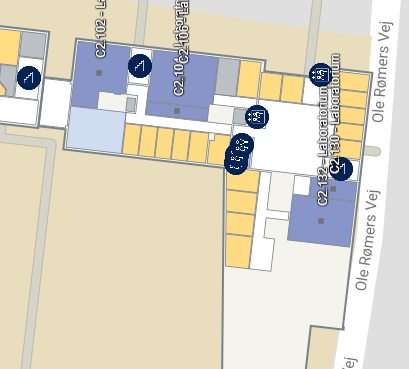
\includegraphics[width=0.4\textwidth]{figures/map/floorplan_aau.png}%
        \label{sub:orient}
        }%
    \hspace{0.1\textwidth}
    \subfloat[School layout example]{%
        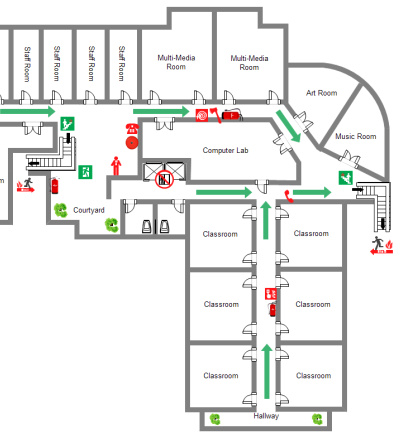
\includegraphics[width=0.4\textwidth]{figures/map/floorplan_school.png}%
        \label{sub:evac}
        }%
    \caption{Examples of different maps}
    \label{fig:floor_plans}
\end{figure}
% https://www.edrawsoft.com/school-layout-example.php

Maps are often very visual, providing a lot of detailed information to the reader.
The way the information is represented differently,
makes it very hard for a computer to interpret.
A map must provide necessary information,
in a way that can be interpreted by the micro controller.
For this project we decided that a simplified map, would be sufficient.

Table \ref{table:map_data} shows which data the map should include,
as well as some areas that have been delimited from.

\begin{table}[h!]
	\centering
	\caption{Map data}
	\begin{tabular}{|p{0.4\textwidth}|p{0.4\textwidth}|}
		\hline
		Data to be included & Data to delimit from \\ 
		\hline
		Map dimensions 		& \parbox[t]{0.4\textwidth}{Differences in height\\(levels, stairs etc.)}\\
		\hline
		Start position 		& Door openings \\
		\hline
		Finish position 	& \parbox[t]{0.4\textwidth}{Ground surface\\(slipping, traction)} \\
		\hline
		Walls 				& Objects\\
		\hline
	\end{tabular}
	\label{table:map_data}
\end{table}

\section{Map Coordinates}
\label{sec:map_coordinates} % section label
During the theoretical development we often used hand-drawn 2D maps with grids, equivalent to the map depicted in Figure \ref{sub:2d_map}. 
The map can have a certain size and allows for an object such as a wall to have a location on the grid. 
A specific part of the map can easily be referred to by its unique coordinate in the x and y dimensions. 

For converting and storing analog maps into a usable digital representation with the same properties, 
we chose to use a 2D array as data structure. 
A 2D array can be thought of as a matrix, where a grid of numbers can be arranged in rows and columns. 
2D arrays are very similar to matrices, and differs in how elements are indexed.

The result of the different indexing methods can be seen by comparing Figure \ref{sub:2d_map} to \ref{sub:2d_array}. 
Given the same index values, the cell referred to would be different, 
as seen in Figure \ref{fig:grid_map_vs_array}.


\begin{figure}[htp]
    \centering
    \subfloat[2D grid map]{%
        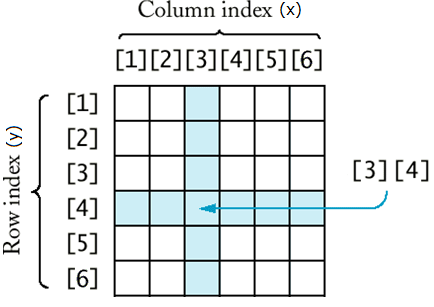
\includegraphics[width=0.45\textwidth]{figures/map/2d-map.png}%
        \label{sub:2d_map}
        }%  
    \hspace{0.05\textwidth}  
    \subfloat[2D array]{%
        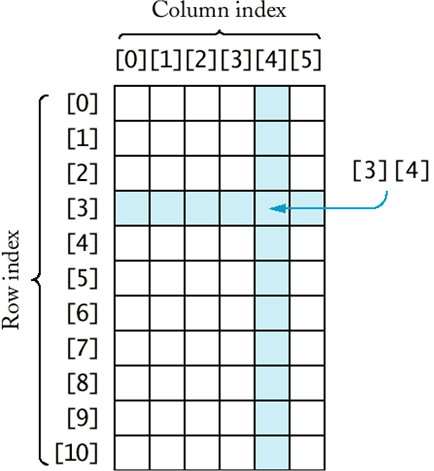
\includegraphics[width=0.45\textwidth]{figures/map/2d-array.png}%
        \label{sub:2d_array}
        }%
    \caption{Difference in indexing for (3,4) in a 2D grid map and a 2D array}
    \label{fig:grid_map_vs_array}
\end{figure}
%https://i.stack.imgur.com/tFdLk.gif

Each cell in the map represents a map segment with its own set of coordinates. 
We chose to start map coordinates at zero, and inf needed rows and columns could still be switched, 
which is very similar to a matrix transpose. 

In the program dynamic 2D arrays were used, 
which allows to easily read or set the value of any given map segment, as shown in Listing \ref{lst:Accessing2dMap}.
The same approach was later used for handling node maps, which is further explained in Chapter \ref{ch:path}.
 
\begin{lstlisting}[caption={Example of reading or setting a value for coordinate (3,4) in the 2D map array, using structs and pointers. Structs are declared in {\tt defs.h} in Appendix X},label={lst:Accessing2dMap}]
robot->map.segments[3][4] = 0x0F;					// Setting a value

char map_segment = robot->map.segments[3][4];	// Reading a value

\end{lstlisting}
\todo{fix ref to appendix}
\section{Map Design}
\label{sec:map_design} % section label
The grid-based map is made up of simple plain-text ASCII characters.
This makes it fairly simple and easy-to-understand, and maps can easily be created or changed by a user. 

An example of a map with 5x5 nodes can be seen in Figure \ref{sub:map_ascii}, 
where \# being walls, A being the start, B being the finish, o being nodes, and the whitespaces being open spaces. 
The same map can be seen using UTF8 encoding in Figure \ref{sub:map_utf8}. 
UTF8 has a more characters to choose from, which makes it easier to read for humans , 
while the plain-text version is easier to read for computers.

Nodes represent positions on the map where the robot can move between, more on nodes in Section \ref{sec:graphs}. 
The robot can move in any of the eight directions unless it is blocked by a wall. 
The directions consists of four straight directions, N,E,S,W and four diagonal directions NE,SE,SW,NW. 
\begin{figure}[htp]
    \centering
    \subfloat[ASCII]{%
        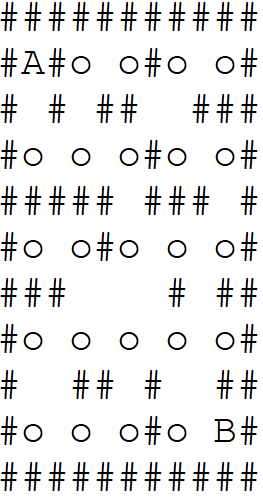
\includegraphics[width=0.2\textwidth]{figures/map/5x5map_ascii-2.png}%
        \label{sub:map_ascii}

    }
    \hspace{0.2\textwidth}
    \subfloat[UTF8]{%
        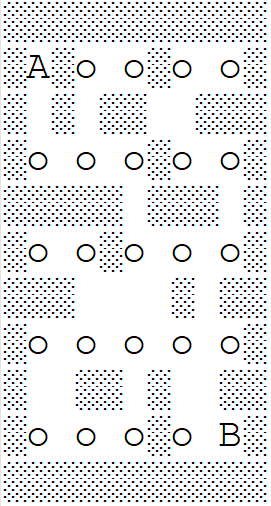
\includegraphics[width=0.2\textwidth]{figures/map/5x5map_utf8-2.png}%
        \label{sub:map_utf8}
    }
    \caption{Example of a map with 5x5 nodes, having 11 characters per line and 11 lines.}
    \label{fig:5x5map}
\end{figure}

We found that making the map using UTF8 would require a bit more work, 
since text editors sometimes add characters to the beginning of the file. 
This is known as the byte-order-mark (BOM) which indicates the file uses UTF8 encoding. 
It also uses variable bit-length for characters, between 1-6 bytes.
This makes reading and storing the map to a file more complicated, which is why we chose to use plain text ASCII.

\newpage
\section{Reading Map from a File}
\label{sec:map_read} % section label %
The function {\tt map\_load} loads map data from a file and saves it in the {\tt map} struct.
Start and finish positions are read from the file as well, and saved in {\tt robot} struct.

Functions were made for loading maps from a text-file, as well as saving an updated map to a text-file. 
The full code for the functions {\tt map\_load} and {\tt map\_save} can be seen in Appendix X.
\todo{fix reference}

Reading and writing maps on a computer locally, was very useful for developing and testing the map handling subsystem. 
Implementing this functionality on a microprocessor, would require it to have a file system installed.
We chose not to implement this functionality, due to the restricted time frame of this project.
As an alternative, maps can be stored directly in memory as part of the programming code. 
This solution is not as user-friendly, and updates to the map will be lost from the memory when the microcontroller is turned off.

In the C programming language the size of an array must be declared at compile time. 
The array for the map has to be large enough to hold all the map data.
Unfortunately the map size and data remains unknown until a map is loaded, which happens during runtime.

One way of dealing with this, is by using a 2D array with a fixed size, large enough to store maps of a convenient size. 
We chose to use a dynamic 2D array instead. 
This more advanced approach gave us more experience, by using dynamic memory allocation and pointers to implement this solution in the application.
\newpage
The required size of the dynamic 2D array can be calculated by counting the the rows and columns of the map,
which is equivalent to the lines and characters.
A map with 5x5 nodes will have 11 characters in each line and a total of 11 lines,
as illustrated in Figure \ref{fig:5x5map}. Listing \ref{lst:mapHload} shows how a map is read from a text-file, and how the lines and characters are counted.

\lstinputlisting
[firstline=30,			%starts reading the file from line 11
%firstnumber=11,		%starts counting the lines in pdf from 11
lastline=46,			%stops reading the file at line 18
label=lst:mapHload,		%label
caption={Reading map text-file and analysing the map size in {\tt map.c}}
]{code/map.c}
To store the map, an 11x11 2D array is required.
Now that the required array size is known, it can be allocated in the memory as shown in Listing \ref{lst:mapHarrayAllocate}.

\lstinputlisting
[firstline=48,			%starts reading the file from line 11
%firstnumber=11,		%starts counting the lines in pdf from 11
lastline=55,			%stops reading the file at line 18
label=lst:mapHarrayAllocate,	%label
caption={Allocation of 2D array in {\tt map.c}}
]{code/map.c}
Once allocated, the address of 2D array is stored in the {\tt robot} struct as a pointer.\\
The size of the map is stored in the {\tt robot} struct as well, for future reference.


\newpage
At this point the 2D map array is filled with the actual map data from file.
Listing \ref{lst:mapHarrayFill} shows how this is done using two for loops.
The robots start and finish location is read from the map as well,
and converted into coordinates for a starting and finish node.

\lstinputlisting
[firstline=56,			%starts reading the file from line 11
%firstnumber=11,		%starts counting the lines in pdf from 11
lastline=76,			%stops reading the file at line 18
label=lst:mapHarrayFill,	%label
caption={Storing values in the 2D array in {\tt map.c}}
]{code/map.c}

Listing \ref{lst:mapHstartFinish} shows how the coordinates for the start and finish nodes are stored in the {\tt robot} struct for future reference. 

\lstinputlisting
[firstline=85,			%starts reading the file from line 11
%firstnumber=11,		%starts counting the lines in pdf from 11
lastline=87,			%stops reading the file at line 18
label=lst:mapHstartFinish,	%label
caption={Storing start and finish position in the {\tt Robot} struct in {\tt map.c}}
]{code/map.c}

\newpage

\section{Building a Node Map}
\label{sec:map_node} % section label
Path finding algorithms operate with a special type of map called a graph.
A graph consists of only nodes and edges, as explained more in detail in Section \ref{sec:graphs}.
The function {\tt node\_map\_load} converts the ordinary map made of ASCII characters, into a map that only consists of nodes.

Like with linked lists, structs can be used as a data structure to store data of different types. 
Listing \ref{lst:mapStructs} shows the data structure created for the '{\tt Nodes} struct' to hold all the necessary data for the individual nodes.

\lstinputlisting
[firstline=24,			%starts reading the file from line 11
%firstnumber=11,		%starts counting the lines in pdf from 11
lastline=31,			%stops reading the file at line 18
label=lst:mapStructs,	%label
caption={data structure of {\tt Nodes} struct in {\tt defs.h}}
]{code/defs.h}
Each {\tt Nodes struct} has pointers to the eight neighbour {\tt Nodes} struct.
This is similar to the principle of having a pointer in a linked list pointing to the next element.
\todo{insert node struct code here showing the node struct?}

A dynamic 2D array is declared using malloc. It holds structs of type {\tt Nodes}, one for each node on the map. 
\lstinputlisting
[firstline=90,			%starts reading the file from line 11
%firstnumber=11,		%starts counting the lines in pdf from 11
lastline=101,			%stops reading the file at line 18
label=lst:mapStructs,	%label
caption={Declaration of node map 2D array used for storing {\tt Nodes} structs in {\tt map.c}}
]{code/map.c}

In the end a pointer to the declared 2D array gets stored in the {\tt Robot } struct.
This allows for easy access to all the data for a given node, just by using the nodes position on the map as the array index values. An example of the usage can be seen in Listing \ref{lst:AccessingNode}. 

\begin{lstlisting}[caption={Example of accessing a node in the node map stored in a 2D array in {\tt map.c}},label={lst:AccessingNode}]
<<<<<<< Updated upstream
robot->map.node[i][j].[name of element in Nodes struct]
=======
robot->map.node[i][j].[name of element in {\tt nodes} struct]
>>>>>>> Stashed changes
\end{lstlisting}

\section{Encoding Walls in a Single-byte Value}
\label{sec:map_hex}
Each node in the map potentially has up to eight neighbour nodes. 
The robot can move to any of the neighbour nodes, unless the path is blocked by a wall.

To represent the possible directions to move in, we decided to use the boolean values '0' and '1'. 
Here '0' would mean it is possible to move in that direction, while '1' means there is a wall.
It is possible to store data about the available directions in 8 bits in total, equivalent to a single byte.

\begin{figure}[htp]
    \centering
<<<<<<< Updated upstream
        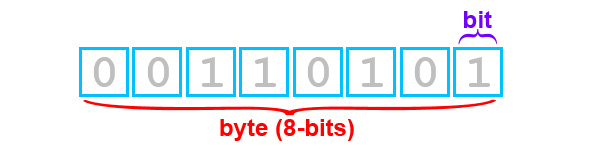
\includegraphics[width=0.70\textwidth]{figures/map/bitbyte.png}%
=======
        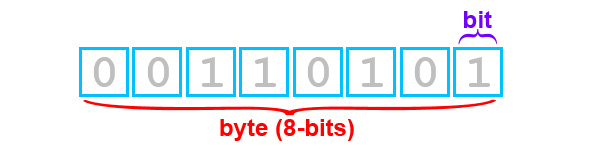
\includegraphics[width=0.75\textwidth]{figures/map/bitbyte.png}%
>>>>>>> Stashed changes
    \caption{A byte where the bit pattern represents the eight possible directions to move in.}
    \label{fig:bitbyte}
\end{figure}

\section{Map Validation Using Sensors}
\label{sec:map_check} % section label
There might be rescuing scenarios where parts of the map, or even the entire map, would be unknown.
External factors such as an explosion in a building, could also change the surroundings dramatically, making the map data invalid.
 
The robots current location on the map is known at all times. 
After the robot has moved to the next node on the map, its current position is updated.
At the robots current location, sensors scans the surrounding environment for walls in the eight possible move-directions.
The feedback from the sensors is returned as a single-byte value, as described in Chapter \ref{ch:scan}.

The single-byte from the {\tt scan} function gets compared to the single-byte in the map array, for the robots current location.
If changes to the surroundings are detected, the 2D map array gets updated and saved to the text-file.
\todo{insert code where char map gets updated based on the scan return and robots current position}

Every time a change in the map is detected, the pathfinding function is called
\todo{insert function name or code}. 
This calculates the most efficient path from the robots current location to the finish, using the updated map data. 
\todo{insert code from map-check function here}
\todo{it could maybe be used somewhere else to explain what the robot does, if not just leave it here.}

\section{Writing Updated Map to a File}
\label{sec:map_save} % section label
Sensors scan the surroundings for walls, at the robots current position.
If changes are detected, the map gets updated as described in Section \ref{sec:map_check}.

If the updated map is kept only in memory, it will be lost once the microcontroller is turned off, since this is not a persistent storage. To prevent this during testing, the map was saved in a text-file.

The individual map segments that consists of ASCII characters, gets written to the map text-file.
This is done by iterating through the entire 2D map array.

\todo{map\_save code}

